\chapter{Introduction}
\label{Chapter1}
\section{Background and Motivation}

% Lasso -> Bayesian Lasso -> Bayesian Lasso Problem -> challenges of Bayesian Lasso -> % Approximate Bayesian Inference(refer to bayesian paradigm) -> Variational Inference -> % motivation

%%%%%%%%%%%%%%%% Next Version
%%%%%%%%%%%%%%%%

%\textbf{Why Bayesian Lasso problem}
%Advantages: 1. Incorporate Variation (inferential quantity), bring prior if we have strong prior, %2. Bayesian: Potential for automatic tuning selection while Freq cross-validation)
%Disadvantages:
%Lasso -> bayesian lasso -> MCMC approximate bayesian inference

\textbf{Introduction of Lasso Problem}\\
The Least Absolute Selection and Shrinkage Operator (Lasso) regression proposed by \cite{tibshirani_1996} belongs to one of the shrinkage methods. As one of the most traditional shrinkage methods, Lasso regression has been proven in Statistical Community over the years.

The Lasso serves two purposes. One is the estimation of regression parameters and the other is the effective shrinking of the coefficients to achieve variable selection purpose, which is also the fundamental difference of Lasso with other methods. The Lasso regression is helpful particularly for high-dimensional because of its sparsity nature.

\textbf{Explain the purpose of Lasso}
The linear regression model is
\begin{equation}
	\label{eq:LRmodel}
	y = \mu 1_n + X\beta + \epsilon.
\end{equation} 

where $\beta$ is a $p*1$ vector of the regression coefficient, y is a $n*1$ vector of the response variable, X is a $n*p$ matrix of covariates, $\mu$ is a $n*1$ vector of the population mean, and $\epsilon$ is the model uncertainty which is distributed normally with mean 0 and variance $\sigma^2$

The Least square estimator suggests the sum of the square of the difference between the estimated response variable and the true response variable should be used as a loss function as described in Equation (\ref{eq:OLS})
\begin{equation}
	\label{eq:OLS}
	\hat{\beta} = \underset{\beta}{\operatorname{argmin}}  (\tilde{y} - X\beta)^T(\tilde{y}-X\beta).
\end{equation}
The tuning parameter $\lambda$ controls the strength of the penalty.
\begin{equation}
	\label{eq:lasso1}
	\hat{\beta}_{lasso} = \underset{\beta}{\operatorname{argmin}} (\tilde{y}-X\beta)^T(\tilde{y}-X\beta) + \lambda ||\beta||_1,
\end{equation}
where $\lambda$ $\geq 0$. $\tilde{y} =  y - \bar{y}\textbf{1}_n$. Larger penalization leads to the more sparse solution of regression coefficient due to a square constraint set resulting from $L_1$ penalty function, resulting in the implicit variable selection of parameter. This can generate a higher prediction accuracy as well as a more interpretable model since we could drop the estimated regression coefficient that has 0 and state they have a weak effect for prediction according to \cite{tibshirani_1996}.
However, due to the non-existence of derivative of absolute value of regression coefficient $\beta$, alternative improved algorithms have been purposed and deployed such as least angle regression (LARS), iterative soft-thresholding, subgradient method, and iteratively reweighted least square (IRLS) by \cite{efron_hastie_johnstone_tibshirani_2004},   \cite{beck_teboulle_2009}, \cite{nan_zhang_shuqing_zeng_2005} and \cite{friedman_hastie_tibshirani_2010}.

\textbf{Bayesian Lasso}
One drawback of the ordinary lasso is that it cannot properly capture the variation of inferential quantity. To address this issue, \cite{tibshirani_1996} suggested extending the lasso estimate under the Bayesian framework. This can be achieved by assigning an independent and identically distributed Laplacian prior from Equation(\ref{eq:MLELasso}) and combining it with the likelihood form in Equation (\ref{eq:LassoPrior}) to obtain the posterior mode Equation(\ref{eq:lassolikelihood}). 
\begin{equation}
	\label{eq:MLELasso}
	\hat{\beta}_{lasso} = \underset{\beta}{\operatorname{argmax}}P(\beta|y,\sigma^2,\tau), \quad \tau = \frac{\lambda}{2\sigma^2}
\end{equation}
\begin{equation}
	\label{eq:LassoPrior}
	f(\beta_j) = (\frac{\tau}{2}) \exp(-\tau|\beta_j|),
\end{equation}
\begin{equation}
	\label{eq:lassolikelihood}
	p(y |\beta,\sigma^2) = N(y|X\beta,\sigma^2I_n).
\end{equation}
% Add full models
\textbf{Introduction of Bayesian Lasso Problem (Why Bayesian Lasso?)}
Nevertheless, there is no tractable integration form for the Bayesian Lasso posterior until \cite{park_casella_2008} further explores the Lasso model under the setting of the Bayesian framework. The choice of a conditional Laplace prior distribution over the regression coefficient $\beta$ conditioning by standard error $\sigma^2$ is added to the Lasso penalty formulation in the frequentist framework. This would ensure the unimodality of full posterior distribution. Based on the closed form of the tractable posterior distribution, a three-step Gibbs sampler is proposed to draw samples from the Bayes Lasso posterior distribution, which can be utilized for further inference of parameters of interest.
There are several benefits to using the Bayesian Lasso model. Firstly, it has easier implementation than the traditional Lasso, although it demands more computation of conditional distribution form is demanded. Secondly, we can generate Bayesian credible intervals simultaneously for the parameters in a model, allowing for the modeling of uncertainty and guiding variable selection.
Thirdly, \cite{park_casella_2008} also state that the Bayesian Lasso model could be a potential solution for addressing the issue of attaining optimal tuning parameter $\lambda$. We can achieve this by using the marginal maximum likelihood method along with a suitable hyperprior, such as a gamma prior on the square of the tuning parameter ($\lambda^2$).
It could support a more stable automatic tuning process of choosing the most appropriate tuning parameter $\lambda$ for the Lasso problem. This is in contrast to the inefficient $K$-fold cross-validation approach under the ordinary Lasso model, which is time-consuming and computationally demanding. Lastly, the three-step Bayesian Lasso Gibbs Sampler proposed by \cite{park_casella_2008} would yield an exact posterior distribution that can be sampled given the exact form of the conditional distribution of each model parameter conditioning on the rest of the other parameters. Theoretically, \cite{khare_hobert_2013} demonstrated a Bayesian Lasso Gibbs sampler version of central limit theorem (CLT), indicating Bayesian Lasso Gibbs sampler satisfies geometric ergodicity for any values of sample size $n \geq 3$ and an arbitrary number of regression coefficient $p$, data matrix $X$, tuning parameter $\lambda$. This means the Bayesian lasso Gibbs sampler is able to achieve asymptotically uncertainty of posterior estimation. To address this issue, \cite{FastBL} invented a reduced step Gibbs sampler instead, successfully accelerating the sampling procedure. 

\textbf{Approxiamte Bayesian Inference Intuition}
The Review of Bayesian inference intuition can be referred from Section \ref{bayeisanP}, but challenges of Bayesian inference motivate the approximate Bayesian inference method thereafter. To be specific, \cite{bishop_2006} states three main challenges of obtaining a posterior distribution. Firstly, the dimension of the target parameter might be high, which results in heavy computational costs for estimating posterior distribution. Secondly, it takes a long time to converge to the target posterior distribution. Thirdly, the computation of the posterior mean parameter $\int_{\theta} \theta p(\theta|\mathcal{D})$ has a high probability without having a simple calculation, resulting in the fact that there might not exist a closed form analytical solution for integration. Much effort has been paid over the years, there are two main types of sampling approaches that are effective currently, which are stochastic sampling algorithms and deterministic approximation algorithms. 

\textbf{Introduction of ABI method}
There are two genres of ABI methods, which include stochastic approaches such as MCMC, where an exact result can be obtained if an infinite computational resource is assigned. Another category lies in deterministic approaches, which provide a faster substitution compared to stochastic approximation approaches.
As stated above, approximate inference methods such as MCMC are used for posterior distribution estimation. The need for approximate Bayesian inference methods arises from the difficulty and impracticality of estimating the exact posterior distribution parameters.

\textbf{Challenges of Bayesian Lasso model}
Three-step Gibbs sampler belongs to the class of MCMC algorithms, which produces samples that demonstrate gradually decreasing correlated samples as the burn-in period is increased. Burn-in period refers to the initial period during which the sample is discarded or ignored to eliminate any potential biases or inconsistencies in the measurement process. The purpose of the burn-in period is to ensure that the measurements are stable and consistent before beginning the actual analysis. The three-step Gibbs sampler is time-consuming and computationally challenging, given the fact that it normally requires a long time to converge inside the interval of acceptable tolerance.

\textbf{Approximation Algorithm: Deterministic type \& VI}.
As mentioned before, due to the limitations of stochastic algorithms, alternative methods such as deterministic Variational Inference (VI) have become popular due to their fast speed and simple computation.
Numerous algorithms have been designed and utilized widely such as VB, Expectation Propagation algorithms, etc. A common variation is the Coordinate Ascent Variational Inference approach produced by \cite{Blei2003LDA}, which assumes that the approximation originates from an analytically tractable class of distribution $Q$. Afterward, it attempts to search for the distribution from this family that is closest to the target posterior distribution with some discrepancy metric, such as the Kullback-Leibler divergence. An optimization-based system in Equation (\ref{eq:VI1}) is established by iteratively updating variational parameters with an appropriate optimization algorithm. A traditional optimization algorithm can be Coordinate Ascent which could obtain approximated posterior distribution in the family of $Q$, while the most common choice is the Normal Distribution due to its simple form and adaptability to other distributions.
To further illustrate the intuition, Figure \ref{fig:VIoptimization} provides further explanation of the aforementioned intuition, goal, and procedure of Variational Inference.

\begin{figure}[H]
	\center
	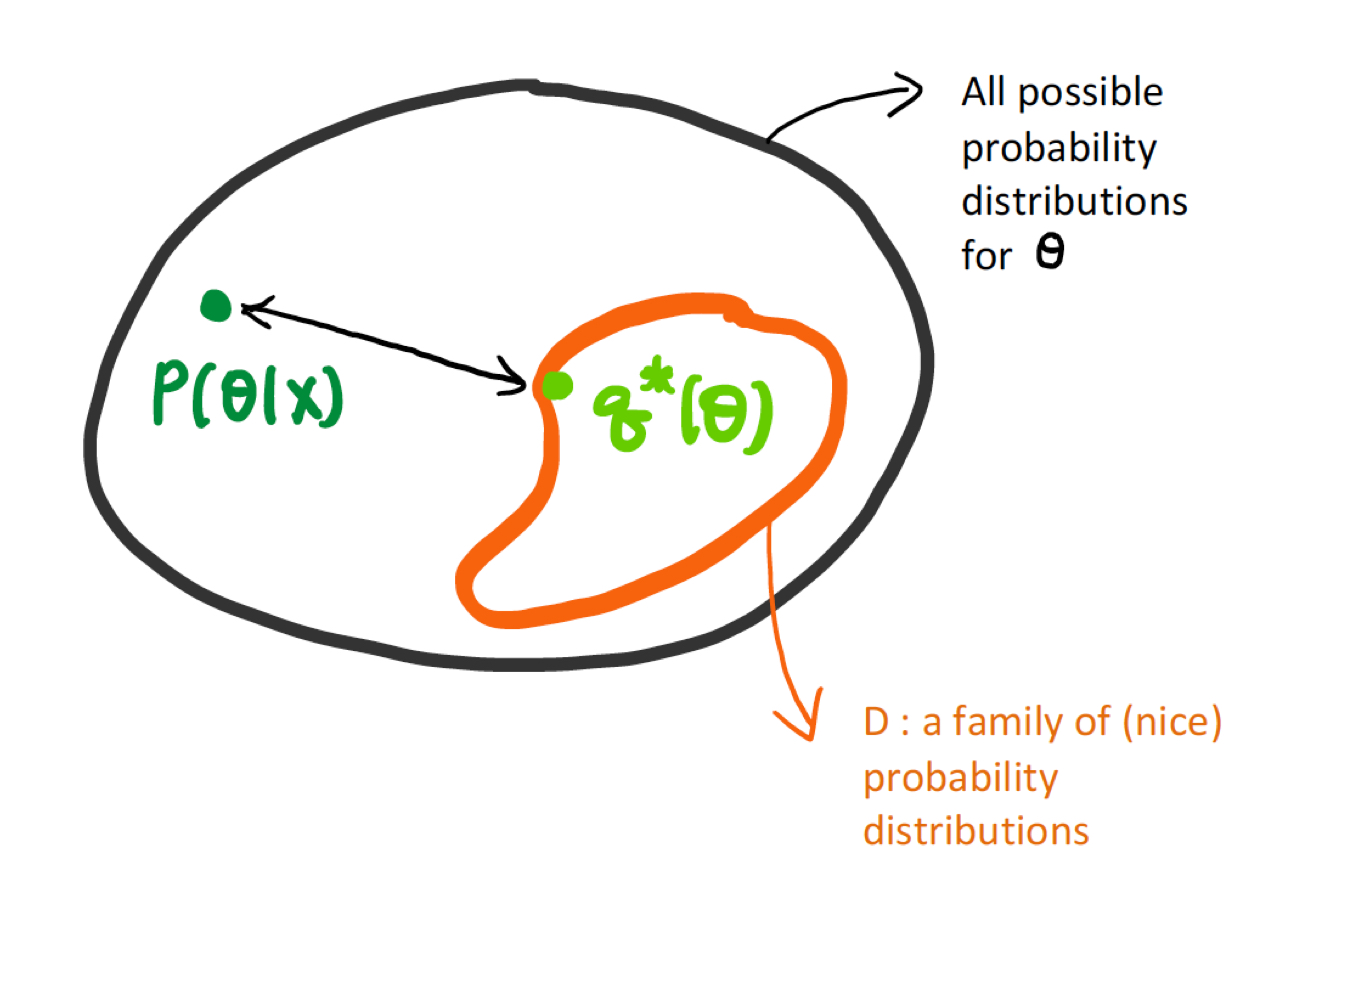
\includegraphics[scale = 0.2]{VIoptimization}
	\caption{Variational Inference intuition, where $X$ is data $\mathcal{D}$, $\mathcal{D}$ is equivalent to $Q$ defined above}
	\label{fig:VIoptimization}
\end{figure}

\begin{equation}
	\label{eq:VI1}
	q^{*}(\theta) = \underset{q_{\theta} \in Q}{\operatorname{argmin}} \textnormal{KL}(q(\theta)||p(\theta|\mathcal{D})) \coloneqq \int q(\theta)\log(\frac{q(\theta)}{p(\theta|\mathcal{D})})d\theta
\end{equation}

\begin{equation}
	\label{eq:KL2}
	\textnormal{KL}(q||p(.|\mathcal{D})) = - \int q(\theta)log(\frac{p(\theta)p(\mathcal{D}|\theta)}{q(\theta)}) d\theta + \log p(\mathcal{D}).
\end{equation}
In addition, the exact form of $\textnormal{KL}$ divergence can be found in Equation (\ref{eq:KL2})
In practice, minimizing the KL divergence from \autoref{eq:VI1} is difficult due to its complexity, and therefore it is often converted into an equivalent formulation in \autoref{eq:KL} that maximizes the lower bound of $\log(p(y))$. This lower bound is known as the Evidence Lower Bound (ELBO) and can be defined by \autoref{eq:KL}).
\begin{equation}
	\label{eq:KL}
	q^*(\theta) = \underset{q_{\theta} \in Q}{\operatorname{ argmax}} \textnormal{ ELBO}(q(\theta)),
\end{equation}
\begin{equation}
	\label{eq:ELBO}	
	\begin{aligned}
		\textnormal{ELBO}(q(\theta)) &= \int q(\theta)\log(\frac{p(\theta)p(\mathcal{D}|\theta)}{q(\theta)}d\theta = \mathop{\mathbb{E}_{q(\theta)}}\log(\frac{p(\theta)p(\mathcal{D}|\theta)}{q(\theta)}).\\
		& = \mathop{\mathbb{E}_{q(\theta)}}[\textnormal{log}p(\theta,\mathcal{D})]
		- \mathop{\mathbb{E}_{q(\theta)}}[\textnormal{log}[q(\theta)]]\\
		&= \mathop{\mathbb{E}_{q(\theta)}}[\textnormal{log}p(\theta,\mathcal{D})]
		- \textnormal{KL}(q(\theta)||p(\theta))\\
	\end{aligned}
\end{equation}

\textbf{Mean Field Variational Bayes, History and Introduction}
% Change reference

The most traditional Variational Inference algorithm is known as MFVB motivated by mean-field theory in statistical physics, as proposed by 
\cite{parisi1988statistical}. The algorithm assumes that the approximated distribution is
a product of independent parameter distributions from set $Q$, as described in \autoref{eq:MFVBassume}, assuming there are $k$ sub-parameters of the target parameter $\theta$.
\begin{equation}
	\label{eq:MFVBassume}
	q(\theta) = \prod_{i=1}^{k} q_i(\theta)
\end{equation}
The MFVBs have been adapted and developed over the last two decades, especially in mixture modeling and probabilistic graphical modeling. It sometimes provides efficient variable selection as well, We will introduce more about the algebra of MFVB in Chapter \ref{Chapter2}. 
\textbf{Advantages of Variational Inference}
One is that the Variational Inference algorithm shows a descent computation cost and scalability, and thus Variational inference can be adaptive when the amount of data is huge. For instance, if there exists a billion image that requires to be fitted into a probabilistic machine learning model, then an exact precision method such as MCMC will be computationally demanding, while Variational Inference would sacrifice tiny accuracy with hundreds of times faster speed as a return.
%Another important factor is that distributed computation and stochastic optimization technique can be embedded in the Variational Inference framework due to its nature of an optimization system, while the Variational Inference originates from Machine Learning for approximating probability density for complex probabilistic graphical model \cite{jordan_ghahramani_jaakkola_saul_1999}. 
Secondly, the descent time-efficiency of Variational Inference becomes another significant factor why it is popular, given the fact it only involves updating variational parameters iteratively until convergence, as opposed to MCMC which produces correlated samples that limit the ideal behavior of the MCMC algorithm.

\textbf{Drawbacks of VI}
Meanwhile, disadvantages of Variational Bayes include inexact approximation results under some scenarios, although it could capture marginal density. For example, it is suggested by \cite{blei_kucukelbir_mcauliffe_2017},
%Might have problem with citation pRML%
that the Variational Inference algorithm might underestimate the covariance between the parameter of interest if the inter-parameter correlation is strong. It tends to ignore the correlation between parameters, resulting in unideal behavior as a result. Figure \ref{fig:VIdemo}
further demonstrates this phenomenon, the true overall posterior of $x_2$ and $x_1$ have an exploded correlation with an eclipse-shaped density, while a circled-shape mean-field approximation is established instead due to its product density family limitation.
\begin{figure}
	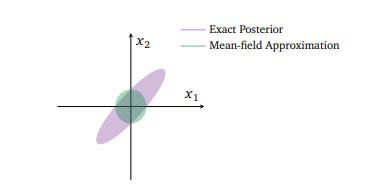
\includegraphics[width=\linewidth]{VIdemo}
	\caption{Visualization of Mean-Field Variational Approximation compared with exact posterior when the correlation is large}
	\label{fig:VIdemo}
\end{figure}
We will expand properties and derivation of Variational Inference more in subsection \ref{VI}.

Overall, Variational Inference has proven its effectiveness in distinct application fields such as speech recognition and document retrieval in natural language processing, computer vision, etc. Despite the small disadvantages of Variational Inference, the potential of variational approximation has not been fully discovered yet by researchers, its ability to provide a reliable posterior estimate is invaluable in the future in the era of big data and deep learning nowadays.

\textbf{Motivation}
This study is motivated by the desire to improve the approximation accuracy of Variational Bayes and to take advantage of the oracle property of Bayesian Lasso regression coefficient estimation for variable selection and standard error estimation, there is an increasing demand for fast approximate inference. We would like to design new VI-based algorithms for the Bayesian Lasso regression problem, for the purpose of obtaining Bayesian Lasso posterior distribution in a much faster and more accurate manner.
We fed the initial values of the mean $\mu$ and covariance $\Sigma$ and wrote out the marginal likelihood form of the regression coefficient $\beta_j$ for the $j_{th}$ variable. Using this information, we invented a new distribution called the univariate Lasso distribution to match the marginal likelihood, represented by $\log(p(\mathcal{D})|\beta_j)$, we have invented a new distribution called univariate lasso distribution for matching the marginal likelihood. Mixing each marginal likelihood with a gaussian approximation. We have demonstrated that our algorithm's approximation accuracy surpasses that of every existing algorithm, including MFVBs. Even though the speed of our algorithm is slightly slower than MFVB, the approximation accuracy illustrates a small gap between exact estimation from MCMC, with a hundred times faster time complexity. Nevertheless, there is a drawback to this method, given the fact that the global covariance matrix would remain diagonal if the initial global covariance matrix is diagonal.
To remedy this issue, we have also purposed another algorithm based on marginal likelihood estimation by a bivariate Lasso distribution. Instead of updating the corresponding mean, and covariance matrix for each variable in each iteration, the marginal likelihood of each pair of variables would be matched, so that further generalize our algorithm. Our conclusions are the univariate Lasso algorithm is faster with a lower accuracy while the bivariate Lasso algorithm is slower with a higher accuracy since it updates each pair of variables at a time resulting in ${p\choose 2}$ of unique pairs. We will show the full intuition and idea later in Chapter \ref{Chapter3}.
By utilizing and fitting both univariate and bivariate Lasso distribution to each of the marginal distributions, an improved estimate for global gaussian approximation can be obtained as defined in Equation (\ref{eq:GV}). Finally, we will show our experiment result in Chapter \ref{Chapter4} using various accuracy metrics.

Our contributions have been listed in the following subsection \ref{cont}.
\begin{equation}
	\label{eq:GV}
	q^{*}(\theta) \approx N(\mu^*,\Sigma^*)
\end{equation}

\section{Contribution}
\label{cont}
Our main contribution could be concluded as the following parts:
\begin{itemize}
	\item Introduction of univariate and multivariate Lasso distribution
	\item Derivation of properties for Univariate Lasso distribution, such as the expectation, variance, cumulative density function form, etc.
	\item Derivation of properties for multivariate Lasso distribution such as the expectation, variance, cumulative density Function form, etc.
	\item Implementation of univariate Lasso distribution and multivariate Lasso distribution property in R.
	\item Design of two new VI approaches based on local approximation by univariate lasso distribution and multivariate lasso distribution respectively.
	\item Conduct of experiment to testify two algorithms under dataset by several evaluation metrics for approximation accuracy such as Hitters dataset etc.
\end{itemize}



\section{Thesis Organization}
The thesis is organized as follows. Chapter 1 briefly illustrates the motivation and background of the Lasso problem, Bayesian Lasso Problem, and Approximate Bayesian Inference, with a specific focus on deterministic Variational Approximation. Chapter 2  briefly reviews and explains the details of the methods in previous work such as the Lasso problem, Approximate Bayesian Inference algorithm, MCMC, Bayesian Expectation Maximization algorithm and their variants, and MFVB. We present our main methodology of the variational algorithm in Chapter 3, followed by a comprehensive experiment for testing the effectiveness of the algorithm in Chapter 4. 



